\documentclass[10pt,a4paper,final]{report}
\usepackage[utf8]{inputenc}
\usepackage[english]{babel}
\usepackage{amsmath}
\usepackage{amsfonts}
\usepackage{amssymb}
\usepackage{float}
\usepackage{fancyhdr}
\usepackage{enumitem}
\usepackage{graphicx}
\usepackage{listings}
\pagestyle{fancy}

\begin{document}
\lstset{language=SQL}
\chead{
Daniel S. Fridjonsson,
Lars Andersen,
S\o ren S. Als \&
Mathias W. Pedersen.
sw608f14 - Room: 2.1.10}


\section*{Self study 1 - miniproject part 1}
Actors, directors, and writers are decided to be stored only as person, since they can preform multiple roles throughout their career. A person has a name, birthday, and additional information. The table for persons will be:

\begin{table}[H] \centering
\begin{tabular}{|c|c|c|}
\hline 
PERSON ID & PERSON NAME & BIRTHDAY \\ 
\hline 
123 & Johnny Known & 03-09-1934 \\ 
\hline 
\end{tabular} 
\end{table}

A movie can contain movie name, movie id, release data, and rating. The rating is calculated by taking the average of the user ratings, see last table, for a specific movie.

\begin{table}[H] \centering
\begin{tabular}{|c|c|c|c|}
\hline 
MOVIE ID & MOVIE NAME & RELEASE DATE & RATING\\ 
\hline 
123 & The Hobbit & 05-12-2014 & 9.2\\ 
\hline 
\end{tabular} 
\end{table}

To connect persons to movies another table is used. Where the role in this table is an enum that contains actor, director, and writer.

\begin{table}[H] \centering
\begin{tabular}{|c|c|c|}
\hline 
MOVIE ID & PERSON ID & ROLE \\ 
\hline 
637 & 463 & Actor \\ 
\hline 
563 & 563 & Director \\ 
\hline 
637 & 674 & Writer \\ 
\hline 
\end{tabular}
\end{table}

Awards can be given to both persons and movies, therefore it is necessary to have two tables, since the id's can be the same for both persons and movies. The tables will be as follows:

\begin{table}[H] \centering
\begin{tabular}{|c|c|c|}
\hline 
MOVIE ID & AWARD & YEAR \\ 
\hline 
542 & Best Picture & 2013 \\ 
\hline 
\end{tabular} 
\end{table}

\begin{table}[H] \centering
\begin{tabular}{|c|c|c|c|}
\hline 
PERSON ID & MOVIE ID & AWARD & YEAR\\ 
\hline 
524 & 542 & Best Actor & 2013 \\ 
\hline 
\end{tabular} 
\end{table}

To store a user of the system it is necessary to store a username and password. The password should be encrypted, but security is not the focus of this exercise.

\begin{table}[H] \centering
\begin{tabular}{|c|c|c|}
\hline 
USER ID & USERNAME & PASSWORD \\ 
\hline 
546 & NiceName & 123456 \\ 
\hline 
\end{tabular} 
\end{table}

Furthermore, a user can rate movies, and a table for this is created. This table contains user id, movie id, and rating

\begin{table}[H] \centering
\begin{tabular}{|c|c|c|}
\hline 
MOVIE ID & USER ID & RATING \\ 
\hline 
634 & 342 & 8 \\ 
\hline 
\end{tabular} 
\end{table}
\newpage
\section*{Self study 2 - miniproject part 2}

\subsection*{ER Diagram}
\begin{figure}[H]
     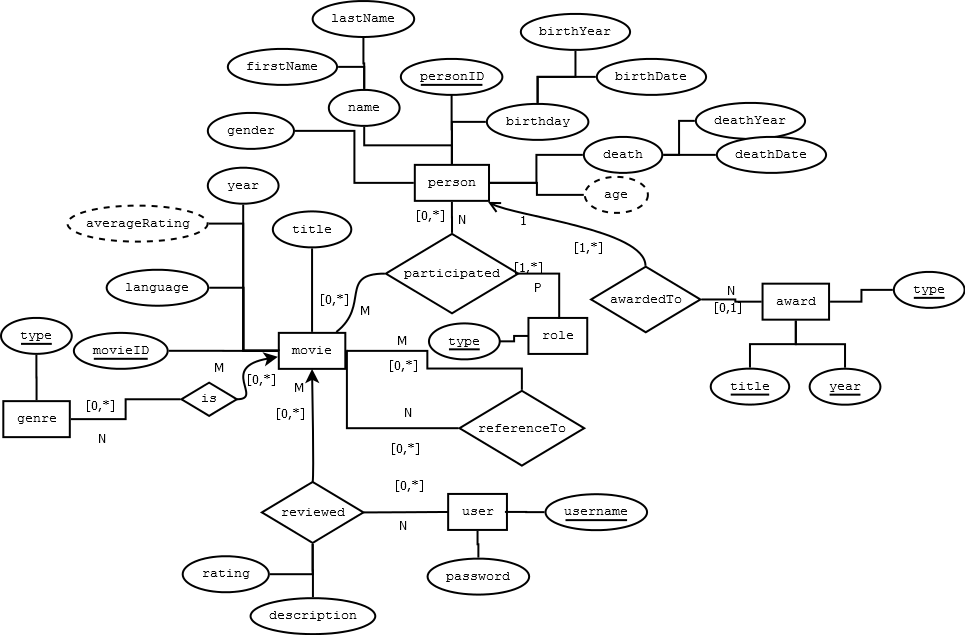
\includegraphics[scale=0.4]{ERdiagram.png}
     \caption{ER Diagram selfstudy 2}
\end{figure}
\subsection*{Relational Schema}
\begin{description}[style=nextline]
     \item[genre]
     $\{[\underline{type:String}]\}$
     \item[movie]
     $\{[\underline{movieID:Int},language:String,year:Int,title:String]\}$
     \item[user]
     $\{[\underline{username:String},password:String]\}$
     \item[award]
     $\{[\underline{title:String, year:Int, type:String}, receiver \rightarrow person]\}$
     \item[person]
     $\{[\underline{personID:Int},firstName:String, lastName:String, gender:String, birthYear:Int, birthDate:String, deathYear:Int, deathDate:String]\}$
     \item[participated]
     $\{[\underline{movieID\rightarrow movie, personID \rightarrow person, type \rightarrow role}]\}$
     \item[is]
     $\{[\underline{type \rightarrow genre, movieID \rightarrow movie}]\}$
     \item[reviewed]
     $\{[\underline{movieID \rightarrow movie, username \rightarrow user}, rating:Int, description:String]\}$
     \item[referenceTo]
     $\{[\underline{from \rightarrow movie, to \rightarrow movie}]\}$
\end{description}

\subsection*{Reflections}
The design is different from the initial design in that the initial design was at a mere table level. Furthermore, several additional attributes have been added to accommodate the expected information requirements.
Another change is that there was no primary and foreign keys highlighted in the original answer.
Average rating in the initial database was intended to be a calculated attribute, but was not listed as such, contrary to the new design.
Additionally we have decided that an award only can be given to a person, as that made the design simpler.
Finally we added the $referenceTo$ relation, as that was a requirement we missed in the first selfstudy.


\section*{Selfstudy 4}
\subsection*{Revised ER Diagram}
\begin{figure}[H]
     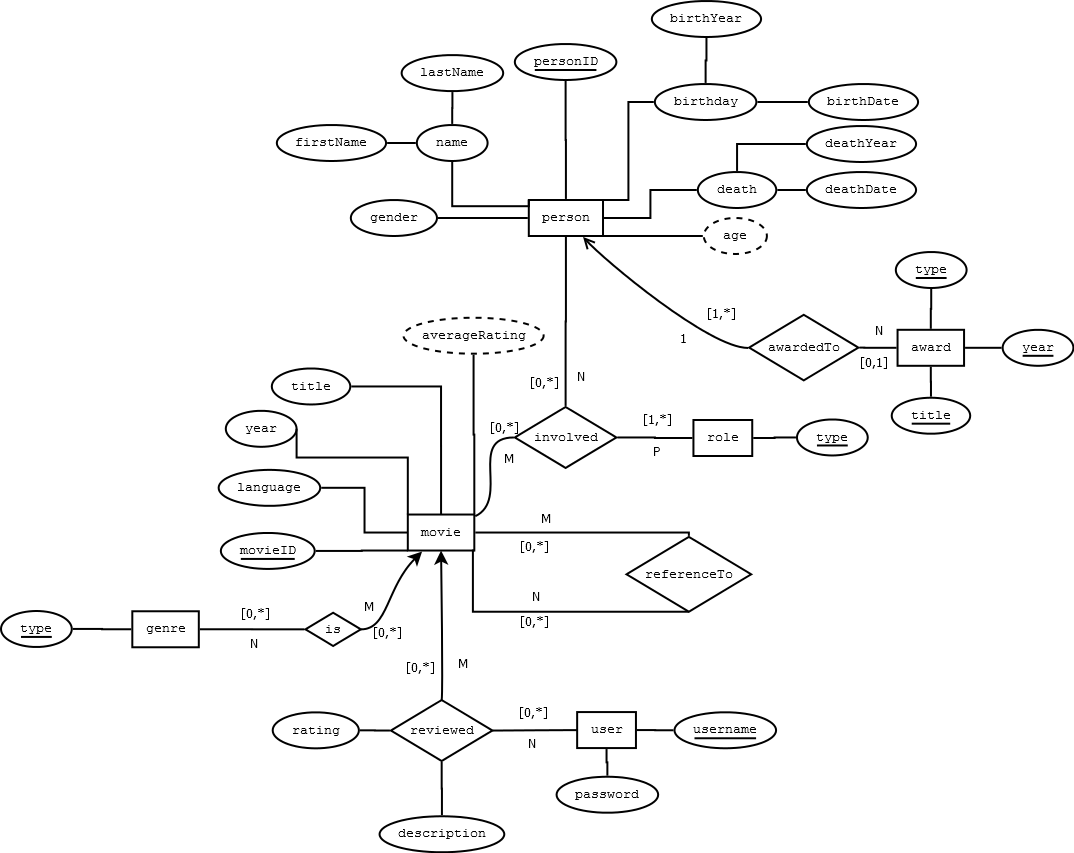
\includegraphics[scale=0.4]{ERdiagramrevisioned}
     \caption{Revised ER Diagram selfstudy 4}
\end{figure}
\subsection*{Revised relational schema}
\subsection*{ER Diagram}
\begin{figure}[h]
     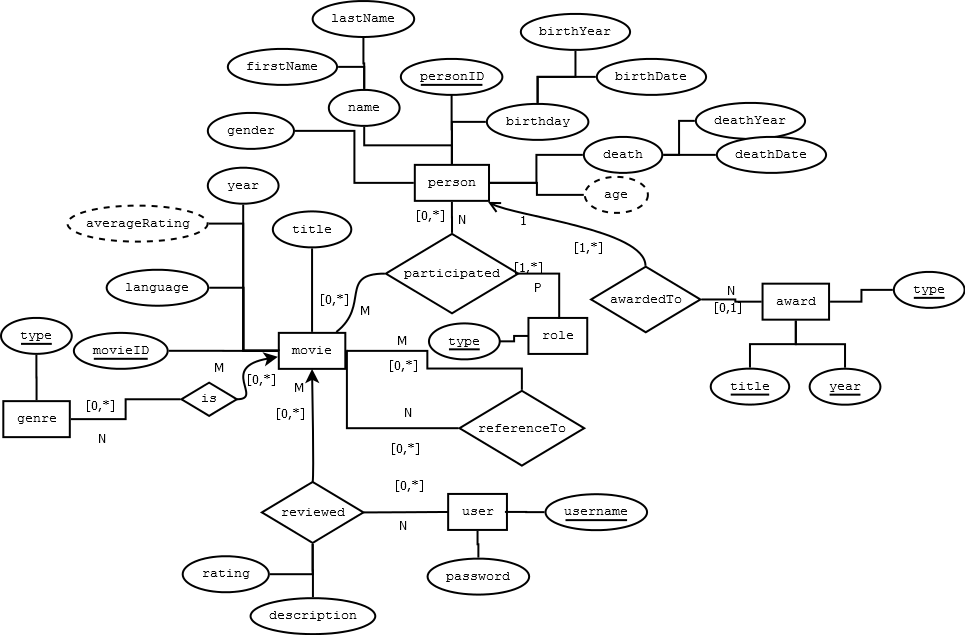
\includegraphics[scale=0.4]{ERdiagram.png}
\end{figure}
\subsection*{Relational Schema}
\begin{description}[style=nextline]
     \item[genre]
     $\{[\underline{type:String}]\}$
     \item[role]
     $\{[\underline{type:String}]\}$
     \item[movie]
     $\{[\underline{movieID:Int},language:String,year:Int,title:String]\}$
     \item[user]
     $\{[\underline{username:String},password:String]\}$
     \item[award]
     $\{[\underline{title:String, year:Int, type:String}, receiver:Int \rightarrow person]\}$
     \item[person]
     $\{[\underline{personID:Int},firstName:String, lastName:String, gender:String, birthYear:Int, birthDate:String, deathYear:Int, deathDate:String]\}$
     \item[involved]
     $\{[\underline{movieID:Int\rightarrow movie, personID:Int \rightarrow person, type:String \rightarrow role}]\}$
     \item[is]
     $\{[\underline{type:String \rightarrow genre, movieID:Int \rightarrow movie}]\}$
     \item[reviewed]
     $\{[\underline{movieID:Int \rightarrow movie, username:String \rightarrow user}, rating:Int, description:String]\}$
     \item[referenceTo]
     $\{[\underline{from:Int \rightarrow movie, to:Int \rightarrow movie}]\}$
\end{description}

\subsection*{Functional Dependencies}

\begin{equation*}
\begin{aligned}
     genre.type &\rightarrow Ø \\
     role.type &\rightarrow Ø \\
     movieID &\rightarrow language, movie.year, movie.title\\
     username  &\rightarrow password \\
     award.title, award.year, award.type &\rightarrow  personID\\
     personID &\rightarrow firstName, lastName, gender, birthYear, birthDate, deathYear, deathDate \\
     movieID, personID, role.type &\rightarrow  Ø \\
     genre.type, movieID &\rightarrow Ø \\     
     movieID, username &\rightarrow rating, description\\
     movieID, movieID &\rightarrow Ø
\end{aligned}
\end{equation*}

It is 3NF as rule 2 applies for all the functional dependencies, since the primary key in each relation is also a super key and due to it being 2NF, as it is fully functionally dependent.
As it is rule 2 that applies for all the functional dependencies, it is also BCNF.

As the schema is already 3NF, there is no need to normalize the relations.

\subsection*{SQL Statements}
\begin{lstlisting}
CREATE TABLE genre
{
     type varchar(15) PRIMARY KEY
};

CREATE TABLE role
{
     type varchar(15) PRIMARY KEY
};


CREATE SEQUENCE serialmovie START 0;

CREATE TABLE movie
{
     movieID integer PRIMARY KEY DEFAULT nextval('serialmovie'),
     language varchar(20) DEFAULT 'English',
     year integer NOT NULL,
     title varchar(100) NOT NULL
};

CREATE TABLE user
{
     username varchar(20) PRIMARY KEY,
     password varchar(50) NOT NULL
};

CREATE TABLE award
{
     title varchar(30),
     year integer,
     type varchar(15),
     receiver integer NOT NULL,
     PRIMARY KEY(title,year,type),
     FOREIGN KEY(receiver) REFERENCES person(personID)
};

CREATE SEQUENCE serialperson START 0;

CREATE TABLE person
{
     personID integer PRIMARY KEY DEFAULT nextval('serialperson'),
     firstName varchar(20) NOT NULL,
     lastName varchar(50) NOT NULL,
     gender varchar(6),
     birthYear integer,
     birthDate varchar(7),
     deathYear integer,
     deathDate varchar(7)
};

CREATE TABLE involved
{
     movieID integer,
     personID integer,
     type varchar(15),
     PRIMARY KEY(movieID, personID, type),
     FOREIGN KEY(movieID) REFERENCES movie(movieID),
     FOREIGN KEY(personID) REFERENCES person(personID),
     FOREIGN KEY(type) REFERENCES role(type)
}

CREATE TABLE is
{
     type varchar(15),
     movieID integer,
     PRIMARY KEY(type,movieID),
     FOREIGN KEY(type) REFERENCES genre(type),
     FOREIGN KEY(movieID) REFERENCES movie(movieID)
};

CREATE TABLE reviewed
{
     movieID integer,
     username varchar(20),
     rating integer NOT NULL,
     description varchar(MAX),
     PRIMARY KEY(movieID, username),
     FOREIGN KEY(movieID) REFERENCES movie(movieID),
     FOREIGN KEY(username) REFERENCES user(username)
};

CREATE TABLE referenceTo
{
     from integer,
     to integer,
     PRIMARY KEY(from, to),
     FOREIGN KEY(from,to) REFERENCES movie(movieID)
};
\end{lstlisting}

\subsection*{Reflections}
Differences from the original design is that we changed the layout of our ER Diagram and renamed the \textit{participated} relation to \textit{involved}.
Considerations we have to take in the future is our encoding of dates, which could be changed to the \textit{DATETIME} datatype.
Also, we forgot the role relation in our first schema, and was thus added to the revised schema.
\end{document}